\chapter{Introduction}
\label{ChapterIntroduction}
%\renewcommand{\baselinestretch}{1.5}\normalsize
%
The parallax effect(Ability to see an object at two different views) is present in stereoscopic or stereo pair image. The objects near the camera will represent more to the right in the left image and more left in the right image is due to parallax effect in stereoscopic or stereo pair   image. 
\begin{figure}[h] 
  % Requires \usepackage{graphicx}
  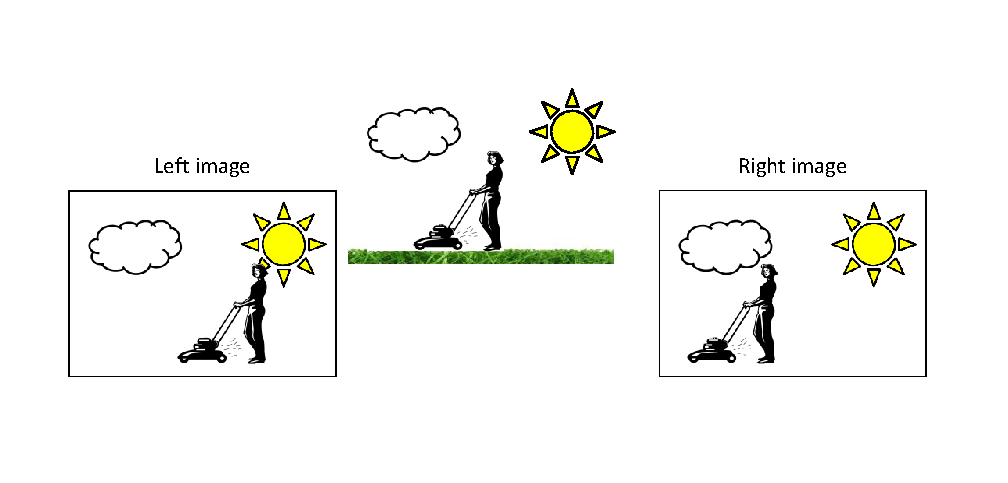
\includegraphics[width=5in]{parallax.eps}
  \caption{Effect of parallax in stereo image } \label{rp}
\end{figure}

To find the horizontal matching pixel in left and right image for stereo pair image is known as stereo vision, stereo correspondence or stereo matching.The horizontal pixel distance for each pixel coordinates is the disparity map or the depth map. The Depth map or Disparity map is a gray scale image which is highly compressed.\\ The Depth map or Disparity map shows distance rather than texture. If shift of pixel between  right and left stereo image is more than object looks darker which is located far away from camera and if shift is less than object is bright i.e. object close to the camera. In practice where occluded objects in stereo pair image, finding the corresponding point or points showing corresponding object is a challenging one which is due to there is no procedure to identify the group of pixel from the same object.
\begin{figure}[h]
  % Requires \usepackage{graphicx}
  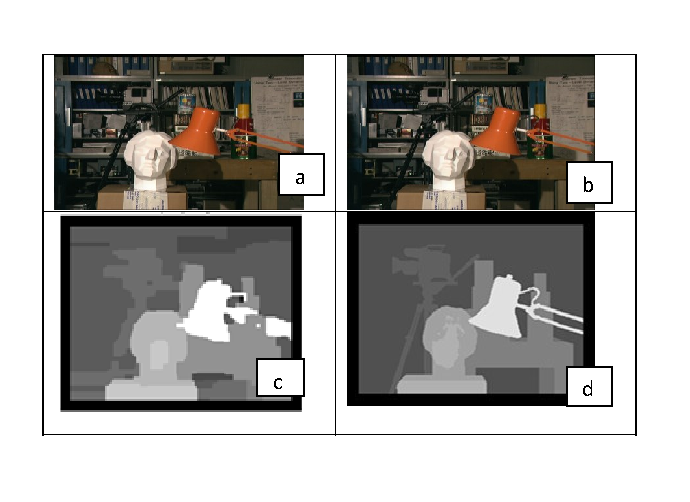
\includegraphics[width=5in]{sampledm.eps}
  \caption{a.Left Image b.Right Image c.Depth Map by BP d.GroundTruth} \label{rp}
\end{figure}
\\ Some applications of Depth Map or Disparity Map  are:\begin{itemize}
                                                       \item {In robot application for navigation purpose and for object recognition to separate occluded image components.} 
                                                       \item {To reconstruct 3D model sequences which can be used either for information transfer or for entertainment or for Image sequence analysis}
                                                       \item {Used for scientific application to extracts information from aerial surveys and for calculation of contour maps }
                                                     \item{  Used as  Gaze correction for video conference}
                                                     \end{itemize}
 Stereo matching Algorithm is classified as Area-based, Feature- based and Global algorithm. The Area and feature based algorithms are based on intensity profile. The constrains in area- based algorithm is to find the optimal size of the window. The feature-based algorithms are restricted to using only specific feature, that only yield sparse disparity maps. However these techniques had limited success.\\
The Belief propagation algorithm is one of the possible inference algorithm based on Bayesian approach to finds corresponding point or points in stereo image as an energy minimization problem. The Belief propagation algorithm is iterative process works well and also computationally simple and computationally efficient for occluded objects.
Organization of report
